\documentclass[12pt]{article}
\usepackage{tikz}
\usepackage{amsmath}
% Underlining package
\usepackage{ulem}
\usetikzlibrary{calc}
\usetikzlibrary{angles,quotes}
\usepackage[a4paper, portrait, margin=1cm]{geometry}
\usepackage{fancyhdr}

\newcommand{\HeadingQuestions}{%
\section*{\Large Name: \underline{\hspace{8cm}} \hfill Date: \underline{\hspace{3cm}}}%
\vspace{-3mm}\par
\textbf{Area of a Circle}\vspace{1pt}\hrule
}

% raise footer with page number; no header
\fancypagestyle{myfancypagestyle}{
  \fancyhf{}% clear all header and footer fields
  \renewcommand{\headrulewidth}{0pt} % no rule under header
  \fancyfoot[C] {\thepage} \setlength{\footskip}{14.5pt} % raise page number allowed min 14.5pt
}
\pagestyle{myfancypagestyle}  % apply myfancypagestyle

\newcounter{minipagecount}

\begin{document}
\HeadingQuestions
\vspace{8mm}

\begin{minipage}{0.50\textwidth}
  \refstepcounter{minipagecount}
  \noindent{(\theminipagecount)}\quad
  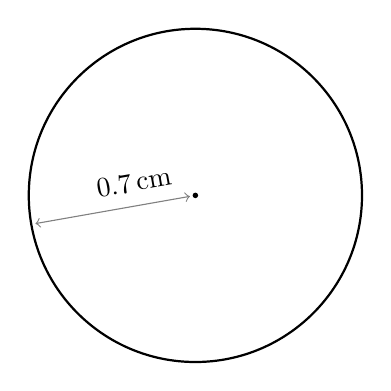
\begin{tikzpicture}[scale=1.0, baseline=(current bounding box.north)]
    \begin{scope}[rotate=0]
        \coordinate (A) at (0,0);
        % Define B using polar coordinates from A
        \coordinate (B) at ($(A) + (190:2.116)$);
        \fill (A) circle(1pt);
        \draw[thick] (A) circle (2.116);
        \draw[<->, gray, shorten <=2pt, shorten >=1.5pt]
          (A) -- (B)
          node[pos=0.35, sloped, above, fill=white, inner sep=2pt, xshift=0pt, yshift=3pt, transform shape]
          {\textcolor{black}{$0.7\,\text{cm}$}};
    \end{scope}
  \end{tikzpicture}
\end{minipage}%
\hfill
\begin{minipage}{0.45\textwidth}
  \begin{align*}
  \text{Circumference} &= 2\pi r \\
  \text{Circumference} &= 2 \times \pi \times \dotuline{~~~~~~~~~~~~}\,\text{cm} \\
  \text{Circumference} &\approx \dotuline{~~~~~~~~~~~~} \,\text{cm}
  \end{align*}
\end{minipage}
\par\vspace{1cm}\begin{minipage}{0.50\textwidth}
  \refstepcounter{minipagecount}
  \noindent{(\theminipagecount)}\quad
  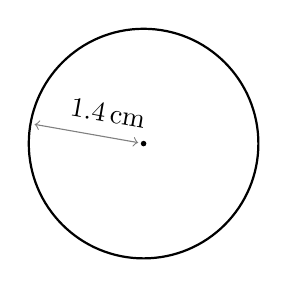
\begin{tikzpicture}[scale=1.0, baseline=(current bounding box.north)]
    \begin{scope}[rotate=0]
        \coordinate (A) at (0,0);
        % Define B using polar coordinates from A
        \coordinate (B) at ($(A) + (170:1.458)$);
        \fill (A) circle(1pt);
        \draw[thick] (A) circle (1.458);
        \draw[<->, gray, shorten <=2pt, shorten >=1.5pt]
          (A) -- (B)
          node[pos=0.35, sloped, above, fill=white, inner sep=2pt, xshift=0pt, yshift=3pt, transform shape]
          {\textcolor{black}{$1.4\,\text{cm}$}};
    \end{scope}
  \end{tikzpicture}
\end{minipage}%
\hfill
\begin{minipage}{0.45\textwidth}
  \begin{align*}
  \text{Circumference} &= 2\pi r \\
  \text{Circumference} &= 2 \times \pi \times \dotuline{~~~~~~~~~~~~}\,\text{cm} \\
  \text{Circumference} &\approx \dotuline{~~~~~~~~~~~~} \,\text{cm}
  \end{align*}
\end{minipage}
\par\vspace{1cm}\begin{minipage}{0.50\textwidth}
  \refstepcounter{minipagecount}
  \noindent{(\theminipagecount)}\quad
  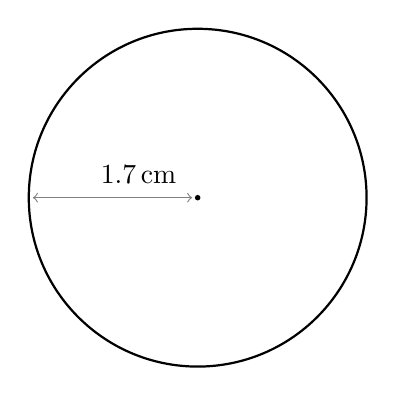
\begin{tikzpicture}[scale=1.0, baseline=(current bounding box.north)]
    \begin{scope}[rotate=0]
        \coordinate (A) at (0,0);
        % Define B using polar coordinates from A
        \coordinate (B) at ($(A) + (180:2.145)$);
        \fill (A) circle(1pt);
        \draw[thick] (A) circle (2.145);
        \draw[<->, gray, shorten <=2pt, shorten >=1.5pt]
          (A) -- (B)
          node[pos=0.35, sloped, above, fill=white, inner sep=2pt, xshift=0pt, yshift=3pt, transform shape]
          {\textcolor{black}{$1.7\,\text{cm}$}};
    \end{scope}
  \end{tikzpicture}
\end{minipage}%
\hfill
\begin{minipage}{0.45\textwidth}
  \begin{align*}
  \text{Circumference} &= 2\pi r \\
  \text{Circumference} &= 2 \times \pi \times \dotuline{~~~~~~~~~~~~}\,\text{cm} \\
  \text{Circumference} &\approx \dotuline{~~~~~~~~~~~~} \,\text{cm}
  \end{align*}
\end{minipage}
\par\vspace{1cm}\begin{minipage}{0.50\textwidth}
  \refstepcounter{minipagecount}
  \noindent{(\theminipagecount)}\quad
  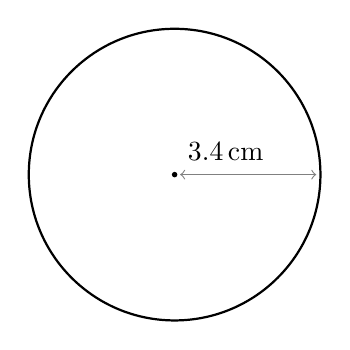
\begin{tikzpicture}[scale=1.0, baseline=(current bounding box.north)]
    \begin{scope}[rotate=0]
        \coordinate (A) at (0,0);
        % Define B using polar coordinates from A
        \coordinate (B) at ($(A) + (0:1.852)$);
        \fill (A) circle(1pt);
        \draw[thick] (A) circle (1.852);
        \draw[<->, gray, shorten <=2pt, shorten >=1.5pt]
          (A) -- (B)
          node[pos=0.35, sloped, above, fill=white, inner sep=2pt, xshift=0pt, yshift=3pt, transform shape]
          {\textcolor{black}{$3.4\,\text{cm}$}};
    \end{scope}
  \end{tikzpicture}
\end{minipage}%
\hfill
\begin{minipage}{0.45\textwidth}
  \begin{align*}
  \text{Circumference} &= 2\pi r \\
  \text{Circumference} &= 2 \times \pi \times \dotuline{~~~~~~~~~~~~}\,\text{cm} \\
  \text{Circumference} &\approx \dotuline{~~~~~~~~~~~~} \,\text{cm}
  \end{align*}
\end{minipage}
\par\vspace{1cm}\begin{minipage}{0.50\textwidth}
  \refstepcounter{minipagecount}
  \noindent{(\theminipagecount)}\quad
  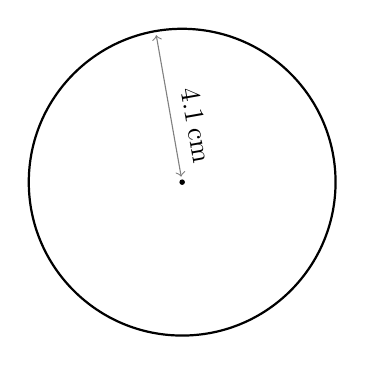
\begin{tikzpicture}[scale=1.0, baseline=(current bounding box.north)]
    \begin{scope}[rotate=0]
        \coordinate (A) at (0,0);
        % Define B using polar coordinates from A
        \coordinate (B) at ($(A) + (100:1.948)$);
        \fill (A) circle(1pt);
        \draw[thick] (A) circle (1.948);
        \draw[<->, gray, shorten <=2pt, shorten >=1.5pt]
          (A) -- (B)
          node[pos=0.35, sloped, above, fill=white, inner sep=2pt, xshift=0pt, yshift=3pt, transform shape]
          {\textcolor{black}{$4.1\,\text{cm}$}};
    \end{scope}
  \end{tikzpicture}
\end{minipage}%
\hfill
\begin{minipage}{0.45\textwidth}
  \begin{align*}
  \text{Circumference} &= 2\pi r \\
  \text{Circumference} &= 2 \times \pi \times \dotuline{~~~~~~~~~~~~}\,\text{cm} \\
  \text{Circumference} &\approx \dotuline{~~~~~~~~~~~~} \,\text{cm}
  \end{align*}
\end{minipage}
\par\vspace{1cm}\begin{minipage}{0.50\textwidth}
  \refstepcounter{minipagecount}
  \noindent{(\theminipagecount)}\quad
  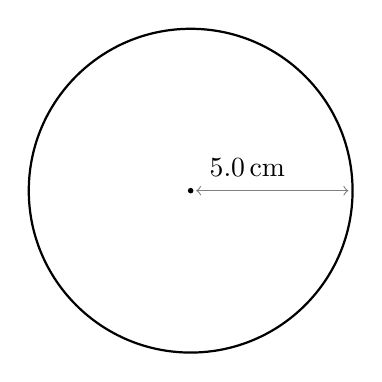
\begin{tikzpicture}[scale=1.0, baseline=(current bounding box.north)]
    \begin{scope}[rotate=0]
        \coordinate (A) at (0,0);
        % Define B using polar coordinates from A
        \coordinate (B) at ($(A) + (0:2.056)$);
        \fill (A) circle(1pt);
        \draw[thick] (A) circle (2.056);
        \draw[<->, gray, shorten <=2pt, shorten >=1.5pt]
          (A) -- (B)
          node[pos=0.35, sloped, above, fill=white, inner sep=2pt, xshift=0pt, yshift=3pt, transform shape]
          {\textcolor{black}{$5.0\,\text{cm}$}};
    \end{scope}
  \end{tikzpicture}
\end{minipage}%
\hfill
\begin{minipage}{0.45\textwidth}
  \begin{align*}
  \text{Circumference} &= 2\pi r \\
  \text{Circumference} &= 2 \times \pi \times \dotuline{~~~~~~~~~~~~}\,\text{cm} \\
  \text{Circumference} &\approx \dotuline{~~~~~~~~~~~~} \,\text{cm}
  \end{align*}
\end{minipage}
\par\vspace{1cm}\begin{minipage}{0.50\textwidth}
  \refstepcounter{minipagecount}
  \noindent{(\theminipagecount)}\quad
  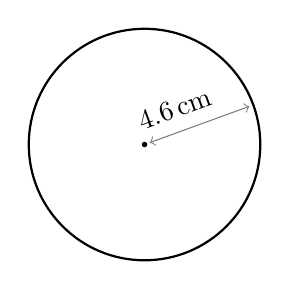
\begin{tikzpicture}[scale=1.0, baseline=(current bounding box.north)]
    \begin{scope}[rotate=0]
        \coordinate (A) at (0,0);
        % Define B using polar coordinates from A
        \coordinate (B) at ($(A) + (20:1.47)$);
        \fill (A) circle(1pt);
        \draw[thick] (A) circle (1.47);
        \draw[<->, gray, shorten <=2pt, shorten >=1.5pt]
          (A) -- (B)
          node[pos=0.35, sloped, above, fill=white, inner sep=2pt, xshift=0pt, yshift=3pt, transform shape]
          {\textcolor{black}{$4.6\,\text{cm}$}};
    \end{scope}
  \end{tikzpicture}
\end{minipage}%
\hfill
\begin{minipage}{0.45\textwidth}
  \begin{align*}
  \text{Circumference} &= 2\pi r \\
  \text{Circumference} &= 2 \times \pi \times \dotuline{~~~~~~~~~~~~}\,\text{cm} \\
  \text{Circumference} &\approx \dotuline{~~~~~~~~~~~~} \,\text{cm}
  \end{align*}
\end{minipage}
\par\vspace{1cm}\begin{minipage}{0.50\textwidth}
  \refstepcounter{minipagecount}
  \noindent{(\theminipagecount)}\quad
  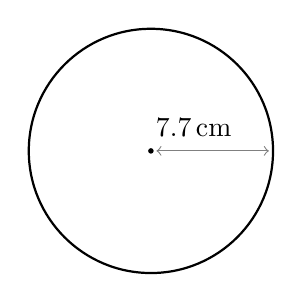
\begin{tikzpicture}[scale=1.0, baseline=(current bounding box.north)]
    \begin{scope}[rotate=0]
        \coordinate (A) at (0,0);
        % Define B using polar coordinates from A
        \coordinate (B) at ($(A) + (0:1.551)$);
        \fill (A) circle(1pt);
        \draw[thick] (A) circle (1.551);
        \draw[<->, gray, shorten <=2pt, shorten >=1.5pt]
          (A) -- (B)
          node[pos=0.35, sloped, above, fill=white, inner sep=2pt, xshift=0pt, yshift=3pt, transform shape]
          {\textcolor{black}{$7.7\,\text{cm}$}};
    \end{scope}
  \end{tikzpicture}
\end{minipage}%
\hfill
\begin{minipage}{0.45\textwidth}
  \begin{align*}
  \text{Circumference} &= 2\pi r \\
  \text{Circumference} &= 2 \times \pi \times \dotuline{~~~~~~~~~~~~}\,\text{cm} \\
  \text{Circumference} &\approx \dotuline{~~~~~~~~~~~~} \,\text{cm}
  \end{align*}
\end{minipage}
\par\vspace{1cm}\begin{minipage}{0.50\textwidth}
  \refstepcounter{minipagecount}
  \noindent{(\theminipagecount)}\quad
  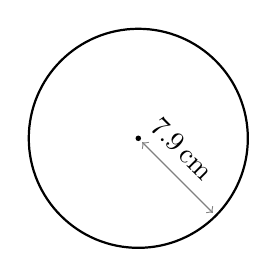
\begin{tikzpicture}[scale=1.0, baseline=(current bounding box.north)]
    \begin{scope}[rotate=0]
        \coordinate (A) at (0,0);
        % Define B using polar coordinates from A
        \coordinate (B) at ($(A) + (315:1.391)$);
        \fill (A) circle(1pt);
        \draw[thick] (A) circle (1.391);
        \draw[<->, gray, shorten <=2pt, shorten >=1.5pt]
          (A) -- (B)
          node[pos=0.35, sloped, above, fill=white, inner sep=2pt, xshift=0pt, yshift=3pt, transform shape]
          {\textcolor{black}{$7.9\,\text{cm}$}};
    \end{scope}
  \end{tikzpicture}
\end{minipage}%
\hfill
\begin{minipage}{0.45\textwidth}
  \begin{align*}
  \text{Circumference} &= 2\pi r \\
  \text{Circumference} &= 2 \times \pi \times \dotuline{~~~~~~~~~~~~}\,\text{cm} \\
  \text{Circumference} &\approx \dotuline{~~~~~~~~~~~~} \,\text{cm}
  \end{align*}
\end{minipage}
\par\vspace{1cm}\begin{minipage}{0.50\textwidth}
  \refstepcounter{minipagecount}
  \noindent{(\theminipagecount)}\quad
  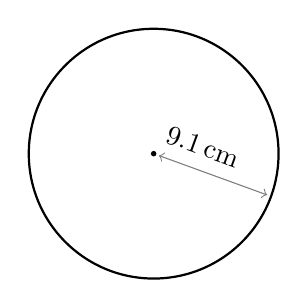
\begin{tikzpicture}[scale=1.0, baseline=(current bounding box.north)]
    \begin{scope}[rotate=0]
        \coordinate (A) at (0,0);
        % Define B using polar coordinates from A
        \coordinate (B) at ($(A) + (-20:1.586)$);
        \fill (A) circle(1pt);
        \draw[thick] (A) circle (1.586);
        \draw[<->, gray, shorten <=2pt, shorten >=1.5pt]
          (A) -- (B)
          node[pos=0.35, sloped, above, fill=white, inner sep=2pt, xshift=0pt, yshift=3pt, transform shape]
          {\textcolor{black}{$9.1\,\text{cm}$}};
    \end{scope}
  \end{tikzpicture}
\end{minipage}%
\hfill
\begin{minipage}{0.45\textwidth}
  \begin{align*}
  \text{Circumference} &= 2\pi r \\
  \text{Circumference} &= 2 \times \pi \times \dotuline{~~~~~~~~~~~~}\,\text{cm} \\
  \text{Circumference} &\approx \dotuline{~~~~~~~~~~~~} \,\text{cm}
  \end{align*}
\end{minipage}
\par\vspace{1cm}\begin{minipage}{0.50\textwidth}
  \refstepcounter{minipagecount}
  \noindent{(\theminipagecount)}\quad
  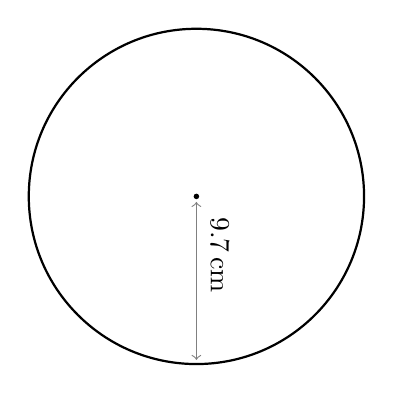
\begin{tikzpicture}[scale=1.0, baseline=(current bounding box.north)]
    \begin{scope}[rotate=0]
        \coordinate (A) at (0,0);
        % Define B using polar coordinates from A
        \coordinate (B) at ($(A) + (270:2.129)$);
        \fill (A) circle(1pt);
        \draw[thick] (A) circle (2.129);
        \draw[<->, gray, shorten <=2pt, shorten >=1.5pt]
          (A) -- (B)
          node[pos=0.35, sloped, above, fill=white, inner sep=2pt, xshift=0pt, yshift=3pt, transform shape]
          {\textcolor{black}{$9.7\,\text{cm}$}};
    \end{scope}
  \end{tikzpicture}
\end{minipage}%
\hfill
\begin{minipage}{0.45\textwidth}
  \begin{align*}
  \text{Circumference} &= 2\pi r \\
  \text{Circumference} &= 2 \times \pi \times \dotuline{~~~~~~~~~~~~}\,\text{cm} \\
  \text{Circumference} &\approx \dotuline{~~~~~~~~~~~~} \,\text{cm}
  \end{align*}
\end{minipage}
\par\vspace{1cm}\begin{minipage}{0.50\textwidth}
  \refstepcounter{minipagecount}
  \noindent{(\theminipagecount)}\quad
  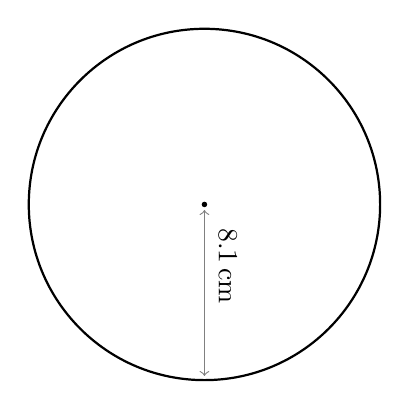
\begin{tikzpicture}[scale=1.0, baseline=(current bounding box.north)]
    \begin{scope}[rotate=0]
        \coordinate (A) at (0,0);
        % Define B using polar coordinates from A
        \coordinate (B) at ($(A) + (270:2.231)$);
        \fill (A) circle(1pt);
        \draw[thick] (A) circle (2.231);
        \draw[<->, gray, shorten <=2pt, shorten >=1.5pt]
          (A) -- (B)
          node[pos=0.35, sloped, above, fill=white, inner sep=2pt, xshift=0pt, yshift=3pt, transform shape]
          {\textcolor{black}{$8.1\,\text{cm}$}};
    \end{scope}
  \end{tikzpicture}
\end{minipage}%
\hfill
\begin{minipage}{0.45\textwidth}
  \begin{align*}
  \text{Circumference} &= 2\pi r \\
  \text{Circumference} &= 2 \times \pi \times \dotuline{~~~~~~~~~~~~}\,\text{cm} \\
  \text{Circumference} &\approx \dotuline{~~~~~~~~~~~~} \,\text{cm}
  \end{align*}
\end{minipage}
\par\vspace{1cm}\begin{minipage}{0.50\textwidth}
  \refstepcounter{minipagecount}
  \noindent{(\theminipagecount)}\quad
  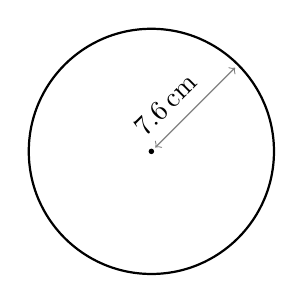
\begin{tikzpicture}[scale=1.0, baseline=(current bounding box.north)]
    \begin{scope}[rotate=0]
        \coordinate (A) at (0,0);
        % Define B using polar coordinates from A
        \coordinate (B) at ($(A) + (45:1.557)$);
        \fill (A) circle(1pt);
        \draw[thick] (A) circle (1.557);
        \draw[<->, gray, shorten <=2pt, shorten >=1.5pt]
          (A) -- (B)
          node[pos=0.35, sloped, above, fill=white, inner sep=2pt, xshift=0pt, yshift=3pt, transform shape]
          {\textcolor{black}{$7.6\,\text{cm}$}};
    \end{scope}
  \end{tikzpicture}
\end{minipage}%
\hfill
\begin{minipage}{0.45\textwidth}
  \begin{align*}
  \text{Circumference} &= 2\pi r \\
  \text{Circumference} &= 2 \times \pi \times \dotuline{~~~~~~~~~~~~}\,\text{cm} \\
  \text{Circumference} &\approx \dotuline{~~~~~~~~~~~~} \,\text{cm}
  \end{align*}
\end{minipage}
\par\vspace{1cm}\begin{minipage}{0.50\textwidth}
  \refstepcounter{minipagecount}
  \noindent{(\theminipagecount)}\quad
  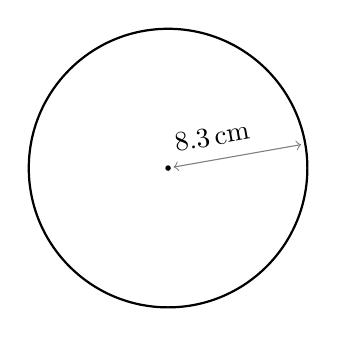
\begin{tikzpicture}[scale=1.0, baseline=(current bounding box.north)]
    \begin{scope}[rotate=0]
        \coordinate (A) at (0,0);
        % Define B using polar coordinates from A
        \coordinate (B) at ($(A) + (10:1.769)$);
        \fill (A) circle(1pt);
        \draw[thick] (A) circle (1.769);
        \draw[<->, gray, shorten <=2pt, shorten >=1.5pt]
          (A) -- (B)
          node[pos=0.35, sloped, above, fill=white, inner sep=2pt, xshift=0pt, yshift=3pt, transform shape]
          {\textcolor{black}{$8.3\,\text{cm}$}};
    \end{scope}
  \end{tikzpicture}
\end{minipage}%
\hfill
\begin{minipage}{0.45\textwidth}
  \begin{align*}
  \text{Circumference} &= 2\pi r \\
  \text{Circumference} &= 2 \times \pi \times \dotuline{~~~~~~~~~~~~}\,\text{cm} \\
  \text{Circumference} &\approx \dotuline{~~~~~~~~~~~~} \,\text{cm}
  \end{align*}
\end{minipage}
\par\vspace{1cm}\begin{minipage}{0.50\textwidth}
  \refstepcounter{minipagecount}
  \noindent{(\theminipagecount)}\quad
  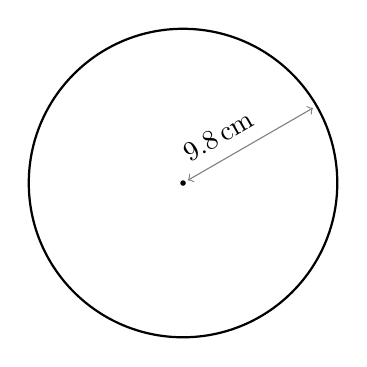
\begin{tikzpicture}[scale=1.0, baseline=(current bounding box.north)]
    \begin{scope}[rotate=0]
        \coordinate (A) at (0,0);
        % Define B using polar coordinates from A
        \coordinate (B) at ($(A) + (30:1.959)$);
        \fill (A) circle(1pt);
        \draw[thick] (A) circle (1.959);
        \draw[<->, gray, shorten <=2pt, shorten >=1.5pt]
          (A) -- (B)
          node[pos=0.35, sloped, above, fill=white, inner sep=2pt, xshift=0pt, yshift=3pt, transform shape]
          {\textcolor{black}{$9.8\,\text{cm}$}};
    \end{scope}
  \end{tikzpicture}
\end{minipage}%
\hfill
\begin{minipage}{0.45\textwidth}
  \begin{align*}
  \text{Circumference} &= 2\pi r \\
  \text{Circumference} &= 2 \times \pi \times \dotuline{~~~~~~~~~~~~}\,\text{cm} \\
  \text{Circumference} &\approx \dotuline{~~~~~~~~~~~~} \,\text{cm}
  \end{align*}
\end{minipage}
\par\vspace{1cm}\begin{minipage}{0.50\textwidth}
  \refstepcounter{minipagecount}
  \noindent{(\theminipagecount)}\quad
  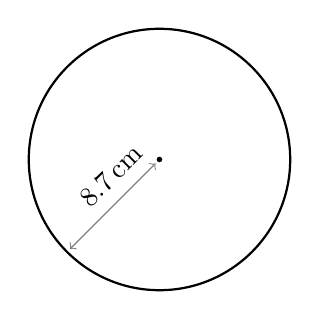
\begin{tikzpicture}[scale=1.0, baseline=(current bounding box.north)]
    \begin{scope}[rotate=0]
        \coordinate (A) at (0,0);
        % Define B using polar coordinates from A
        \coordinate (B) at ($(A) + (225:1.66)$);
        \fill (A) circle(1pt);
        \draw[thick] (A) circle (1.66);
        \draw[<->, gray, shorten <=2pt, shorten >=1.5pt]
          (A) -- (B)
          node[pos=0.35, sloped, above, fill=white, inner sep=2pt, xshift=0pt, yshift=3pt, transform shape]
          {\textcolor{black}{$8.7\,\text{cm}$}};
    \end{scope}
  \end{tikzpicture}
\end{minipage}%
\hfill
\begin{minipage}{0.45\textwidth}
  \begin{align*}
  \text{Circumference} &= 2\pi r \\
  \text{Circumference} &= 2 \times \pi \times \dotuline{~~~~~~~~~~~~}\,\text{cm} \\
  \text{Circumference} &\approx \dotuline{~~~~~~~~~~~~} \,\text{cm}
  \end{align*}
\end{minipage}
\par\vspace{1cm}\begin{minipage}{0.50\textwidth}
  \refstepcounter{minipagecount}
  \noindent{(\theminipagecount)}\quad
  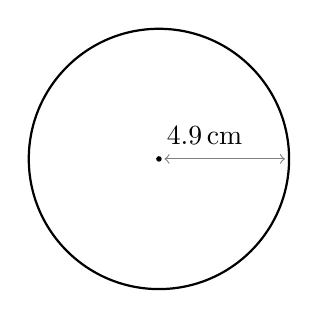
\begin{tikzpicture}[scale=1.0, baseline=(current bounding box.north)]
    \begin{scope}[rotate=0]
        \coordinate (A) at (0,0);
        % Define B using polar coordinates from A
        \coordinate (B) at ($(A) + (0:1.653)$);
        \fill (A) circle(1pt);
        \draw[thick] (A) circle (1.653);
        \draw[<->, gray, shorten <=2pt, shorten >=1.5pt]
          (A) -- (B)
          node[pos=0.35, sloped, above, fill=white, inner sep=2pt, xshift=0pt, yshift=3pt, transform shape]
          {\textcolor{black}{$4.9\,\text{cm}$}};
    \end{scope}
  \end{tikzpicture}
\end{minipage}%
\hfill
\begin{minipage}{0.45\textwidth}
  \begin{align*}
  \text{Circumference} &= 2\pi r \\
  \text{Circumference} &= 2 \times \pi \times \dotuline{~~~~~~~~~~~~}\,\text{cm} \\
  \text{Circumference} &\approx \dotuline{~~~~~~~~~~~~} \,\text{cm}
  \end{align*}
\end{minipage}
\par\vspace{1cm}\begin{minipage}{0.50\textwidth}
  \refstepcounter{minipagecount}
  \noindent{(\theminipagecount)}\quad
  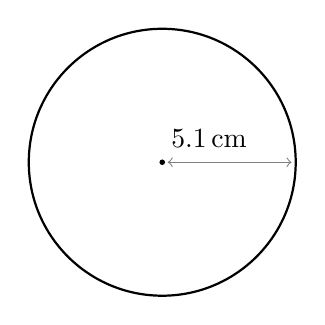
\begin{tikzpicture}[scale=1.0, baseline=(current bounding box.north)]
    \begin{scope}[rotate=0]
        \coordinate (A) at (0,0);
        % Define B using polar coordinates from A
        \coordinate (B) at ($(A) + (0:1.695)$);
        \fill (A) circle(1pt);
        \draw[thick] (A) circle (1.695);
        \draw[<->, gray, shorten <=2pt, shorten >=1.5pt]
          (A) -- (B)
          node[pos=0.35, sloped, above, fill=white, inner sep=2pt, xshift=0pt, yshift=3pt, transform shape]
          {\textcolor{black}{$5.1\,\text{cm}$}};
    \end{scope}
  \end{tikzpicture}
\end{minipage}%
\hfill
\begin{minipage}{0.45\textwidth}
  \begin{align*}
  \text{Circumference} &= 2\pi r \\
  \text{Circumference} &= 2 \times \pi \times \dotuline{~~~~~~~~~~~~}\,\text{cm} \\
  \text{Circumference} &\approx \dotuline{~~~~~~~~~~~~} \,\text{cm}
  \end{align*}
\end{minipage}
\par\vspace{1cm}\begin{minipage}{0.50\textwidth}
  \refstepcounter{minipagecount}
  \noindent{(\theminipagecount)}\quad
  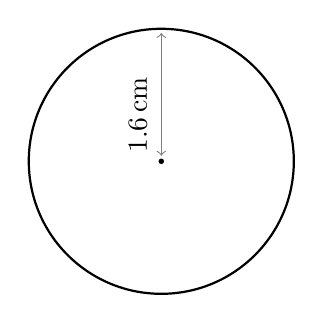
\begin{tikzpicture}[scale=1.0, baseline=(current bounding box.north)]
    \begin{scope}[rotate=0]
        \coordinate (A) at (0,0);
        % Define B using polar coordinates from A
        \coordinate (B) at ($(A) + (90:1.683)$);
        \fill (A) circle(1pt);
        \draw[thick] (A) circle (1.683);
        \draw[<->, gray, shorten <=2pt, shorten >=1.5pt]
          (A) -- (B)
          node[pos=0.35, sloped, above, fill=white, inner sep=2pt, xshift=0pt, yshift=3pt, transform shape]
          {\textcolor{black}{$1.6\,\text{cm}$}};
    \end{scope}
  \end{tikzpicture}
\end{minipage}%
\hfill
\begin{minipage}{0.45\textwidth}
  \begin{align*}
  \text{Circumference} &= 2\pi r \\
  \text{Circumference} &= 2 \times \pi \times \dotuline{~~~~~~~~~~~~}\,\text{cm} \\
  \text{Circumference} &\approx \dotuline{~~~~~~~~~~~~} \,\text{cm}
  \end{align*}
\end{minipage}
\par\vspace{1cm}\begin{minipage}{0.50\textwidth}
  \refstepcounter{minipagecount}
  \noindent{(\theminipagecount)}\quad
  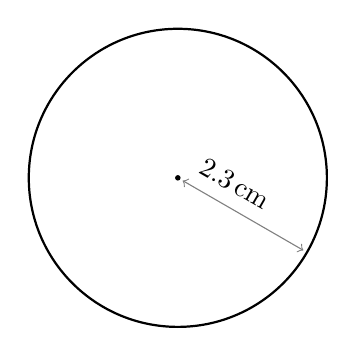
\begin{tikzpicture}[scale=1.0, baseline=(current bounding box.north)]
    \begin{scope}[rotate=0]
        \coordinate (A) at (0,0);
        % Define B using polar coordinates from A
        \coordinate (B) at ($(A) + (-30:1.893)$);
        \fill (A) circle(1pt);
        \draw[thick] (A) circle (1.893);
        \draw[<->, gray, shorten <=2pt, shorten >=1.5pt]
          (A) -- (B)
          node[pos=0.35, sloped, above, fill=white, inner sep=2pt, xshift=0pt, yshift=3pt, transform shape]
          {\textcolor{black}{$2.3\,\text{cm}$}};
    \end{scope}
  \end{tikzpicture}
\end{minipage}%
\hfill
\begin{minipage}{0.45\textwidth}
  \begin{align*}
  \text{Circumference} &= 2\pi r \\
  \text{Circumference} &= 2 \times \pi \times \dotuline{~~~~~~~~~~~~}\,\text{cm} \\
  \text{Circumference} &\approx \dotuline{~~~~~~~~~~~~} \,\text{cm}
  \end{align*}
\end{minipage}
\par\vspace{1cm}

\end{document}
